% Created 2020-06-24 mer. 16:28
% Intended LaTeX compiler: pdflatex
\documentclass{ISMA_USD2020}
\usepackage[utf8]{inputenc}
\usepackage[T1]{fontenc}
\usepackage{graphicx}
\usepackage{grffile}
\usepackage{longtable}
\usepackage{wrapfig}
\usepackage{rotating}
\usepackage[normalem]{ulem}
\usepackage{amsmath}
\usepackage{textcomp}
\usepackage{amssymb}
\usepackage{capt-of}
\usepackage{hyperref}
\usepackage[most]{tcolorbox}
\usepackage{bm}
\usepackage{booktabs}
\usepackage{tabularx}
\usepackage{array}
\usepackage{siunitx}
\usepackage{amsmath,amssymb,amsfonts, cases}
\usepackage{algorithmic, graphicx, textcomp}
\usepackage{xcolor, import, hyperref}
\usepackage{subcaption}
\usepackage[USenglish, english]{babel}
\setcounter{footnote}{1}
\input{config.tex}
\author[1,3] {T. Dehaeze}
\author[1,2] {C. Collette}
\affil[1] {Precision Mechatronics Laboratory\NewLineAffil University of Liege, Belgium \NewAffil}
\affil[2] {BEAMS Department\NewLineAffil Free University of Brussels, Belgium \NewAffil}
\affil[3] {European Synchrotron Radiation Facility \NewLineAffil Grenoble, France e-mail: \textbf{thomas.dehaeze@esrf.fr}}
\bibliographystyle{IEEEtran}
\usepackage{tikz}
\usetikzlibrary{shapes.misc}
\date{}
\title{Active Damping of Rotating Positioning Platforms}
\begin{document}

\maketitle

\abstract{
    Abstract text to be done
}

\section{Introduction}
\label{sec:org3cbd2ff}
\label{sec:introduction}
Controller Poles are shown by black crosses (

\begin{tikzpicture} \node[cross out, draw=black, minimum size=1ex, line width=2pt, inner sep=0pt, outer sep=0pt] at (0, 0){}; \end{tikzpicture}
).
This paper has been published
The Matlab code that was use to obtain the results are available in \cite{dehaeze20_activ_dampin_rotat_posit_platf}.

\section{Dynamics of Rotating Positioning Platforms}
\label{sec:org3cf58d1}
\subsection{Studied Rotating Positioning Platform}
\label{sec:orgf321431}
Consider the rotating X-Y stage of Figure \ref{fig:system}.

\begin{itemize}
\item \(k\): Actuator's Stiffness [N/m]
\item \(m\): Payload's mass [kg]
\item \(\Omega = \dot{\theta}\): rotation speed [rad/s]
\item \(F_u\), \(F_v\)
\item \(d_u\), \(d_v\)
\end{itemize}

\begin{figure}[htbp]
\centering
\includegraphics[scale=1]{figs/system.pdf}
\caption{\label{fig:system}Schematic of the studied System}
\end{figure}


\subsection{Equation of Motion}
\label{sec:org9612ace}
The system has two degrees of freedom and is thus fully described by the generalized coordinates \(u\) and \(v\) (describing the position of the mass in the rotating frame).

Let's express the kinetic energy \(T\) and the potential energy \(V\) of the mass \(m\) (neglecting the rotational energy):

Dissipation function \(R\)
Kinetic energy \(T\)
Potential energy \(V\)
\begin{subequations}
  \begin{align}
    T & = \frac{1}{2} m \left( \left( \dot{u} - \Omega v \right)^2 + \left( \dot{v} + \Omega u \right)^2 \right) \\
    R & = \frac{1}{2} c \left( \dot{u}^2 + \dot{v}^2 \right) \\
    V & = \frac{1}{2} k \left( u^2 + v^2 \right)
  \end{align}
\end{subequations}

The Lagrangian is the kinetic energy minus the potential energy:
\begin{equation}
L = T - V
\end{equation}

From the Lagrange's equations of the second kind, the equation of motion is obtained (\(q_1 = u\), \(q_2 = v\)).
\begin{equation}
  \frac{d}{dt} \left( \frac{\partial L}{\partial \dot{q}_i} \right) + \frac{\partial D}{\partial \dot{q}_i} - \frac{\partial L}{\partial q_i} = Q_i
\end{equation}
with \(Q_i\) is the generalized force associated with the generalized variable \(q_i\) (\(Q_1 = F_u\) and \(Q_2 = F_v\)).


\begin{subequations}
  \begin{align}
    m \ddot{u} + c \dot{u} + ( k - m \Omega ) u &= F_u + 2 m \Omega \dot{v} \\
    m \ddot{v} + c \dot{v} + ( k \underbrace{-\,m \Omega}_{\text{Centrif.}} ) v &= F_v \underbrace{-\,2 m \Omega \dot{u}}_{\text{Coriolis}}
  \end{align}
\end{subequations}

\begin{itemize}
\item Coriolis Forces: coupling
\item Centrifugal forces: negative stiffness
\end{itemize}

Without the coupling terms, each equation is the equation of a one degree of freedom mass-spring system with mass \(m\) and stiffness \(k- m\dot{\theta}^2\).
Thus, the term \(- m\dot{\theta}^2\) acts like a negative stiffness (due to \textbf{centrifugal forces}).


\subsection{Transfer Functions in the Laplace domain}
\label{sec:org1590670}

\begin{subequations}
  \begin{align}
    u &= \frac{ms^2 + cs + k - m \Omega^2}{\left( m s^2 + cs + k - m \Omega^2 \right)^2 + \left( 2 m \Omega s \right)^2} F_u +  \frac{2 m \Omega s}{\left( m s^2 + cs + k - m \Omega^2 \right)^2 + \left( 2 m \Omega s \right)^2} F_v \\
    v &= \frac{-2 m \Omega s}{\left( m s^2 + cs + k - m \Omega^2 \right)^2 + \left( 2 m \Omega s \right)^2} F_u +  \frac{ms^2 + cs + k - m \Omega^2}{\left( m s^2 + cs + k - m \Omega^2 \right)^2 + \left( 2 m \Omega s \right)^2} F_v
  \end{align}
\end{subequations}

\begin{equation}
\begin{bmatrix} d_u \\ d_v \end{bmatrix} =
\bm{G}_d
\begin{bmatrix} F_u \\ F_v \end{bmatrix}
\end{equation}
Where \(\bm{G}_d\) is a \(2 \times 2\) transfer function matrix.

\begin{equation}
\bm{G}_d = \frac{1}{k} \frac{1}{G_{dp}}
\begin{bmatrix}
   G_{dz} & G_{dc} \\
  -G_{dc} & G_{dz}
\end{bmatrix}
\end{equation}
With:
\begin{subequations}
  \begin{align}
    G_{dp} &= \left( \frac{s^2}{{\omega_0}^2} + 2 \xi \frac{s}{\omega_0} + 1 - \frac{{\Omega}^2}{{\omega_0}^2} \right)^2 + \left( 2 \frac{\Omega}{\omega_0} \frac{s}{\omega_0} \right)^2 \\
    G_{dz} &= \frac{s^2}{{\omega_0}^2} + 2 \xi \frac{s}{\omega_0} + 1 - \frac{{\Omega}^2}{{\omega_0}^2} \\
    G_{dc} &= 2 \frac{\Omega}{\omega_0} \frac{s}{\omega_0}
  \end{align}
\end{subequations}

\begin{itemize}
\item \(\omega_0 = \sqrt{\frac{k}{m}}\): Natural frequency of the mass-spring system in \(\si{\radian/\s}\)
\item \(\xi\) damping ratio
\end{itemize}


\subsection{Constant Rotational Speed}
\label{sec:orgd9375df}
To simplify, let's consider a constant rotational speed \(\dot{\theta} = \Omega\) and thus \(\ddot{\theta} = 0\).

\begin{equation}
\label{eq:coupledplant}
\begin{bmatrix} d_u \\ d_v \end{bmatrix} =
\frac{1}{(m s^2 + (k - m{\omega_0}^2))^2 + (2 m {\omega_0} s)^2}
\begin{bmatrix}
  ms^2 + (k-m{\omega_0}^2) & 2 m \omega_0 s \\
  -2 m \omega_0 s          & ms^2 + (k-m{\omega_0}^2) \\
\end{bmatrix}
\begin{bmatrix} F_u \\ F_v \end{bmatrix}
\end{equation}

\begin{equation}
\label{eq:coupled_plant}
\begin{bmatrix} d_u \\ d_v \end{bmatrix} =
\frac{\frac{1}{k}}{\left( \frac{s^2}{{\omega_0}^2} + (1 - \frac{{\Omega}^2}{{\omega_0}^2}) \right)^2 + \left( 2 \frac{{\Omega} s}{{\omega_0}^2} \right)^2}
\begin{bmatrix}
  \frac{s^2}{{\omega_0}^2} + 1 - \frac{{\Omega}^2}{{\omega_0}^2} & 2 \frac{\Omega s}{{\omega_0}^2} \\
  -2 \frac{\Omega s}{{\omega_0}^2}          & \frac{s^2}{{\omega_0}^2} + 1 - \frac{{\Omega}^2}{{\omega_0}^2} \\
\end{bmatrix}
\begin{bmatrix} F_u \\ F_v \end{bmatrix}
\end{equation}

When the rotation speed is null, the coupling terms are equal to zero and the diagonal terms corresponds to one degree of freedom mass spring system.
\begin{equation}
\label{eq:coupled_plant_no_rot}
\begin{bmatrix} d_u \\ d_v \end{bmatrix} =
\frac{\frac{1}{k}}{\frac{s^2}{{\omega_0}^2} + 1}
\begin{bmatrix}
  1 & 0 \\
  0 & 1
\end{bmatrix}
\begin{bmatrix} F_u \\ F_v \end{bmatrix}
\end{equation}

When the rotation speed in not null, the resonance frequency is duplicated into two pairs of complex conjugate poles.
As the rotation speed increases, one of the two resonant frequency goes to lower frequencies as the other one goes to higher frequencies (Figure \ref{fig:campbell_diagram}).

\begin{figure}[htbp]
\begin{subfigure}[c]{0.4\linewidth}
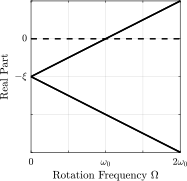
\includegraphics[width=\linewidth]{figs/campbell_diagram_real.pdf}
\caption{\label{fig:campbell_diagram_real} Real Part}
\end{subfigure}
\begin{subfigure}[c]{0.4\linewidth}
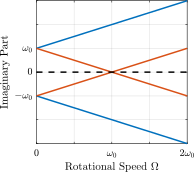
\includegraphics[width=\linewidth]{figs/campbell_diagram_imag.pdf}
\caption{\label{fig:campbell_diagram_imag} Imaginary Part}
\end{subfigure}
\caption{\label{fig:campbell_diagram}Campbell Diagram : Evolution of the poles as a function of the rotational speed \(\Omega\)}
\centering
\end{figure}


The magnitude of the coupling terms are increasing with the rotation speed.

\begin{figure}[htbp]
\begin{subfigure}[c]{0.45\linewidth}
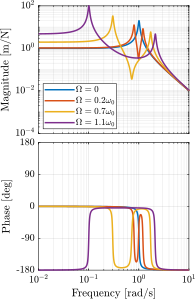
\includegraphics[width=\linewidth]{figs/plant_compare_rotating_speed_direct.pdf}
\caption{\label{fig:plant_compare_rotating_speed_direct} Direct Terms \(d_u/F_u\), \(d_v/F_v\)}
\end{subfigure}
\begin{subfigure}[c]{0.45\linewidth}
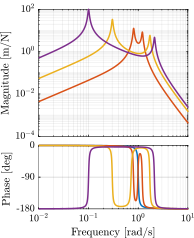
\includegraphics[width=\linewidth]{figs/plant_compare_rotating_speed_coupling.pdf}
\caption{\label{fig:plant_compare_rotating_speed_coupling} Coupling Terms \(d_v/F_u\), \(d_u/F_v\)}
\end{subfigure}
\caption{\label{fig:plant_compare_rotating_speed}Bode Plots for \(\bm{G}_d\)}
\centering
\end{figure}


\section{Integral Force Feedback}
\label{sec:org95f47e8}
\subsection{Control Schematic}
\label{sec:org8bb26ea}

Force Sensors are added in series with the actuators as shown in Figure \ref{fig:system_iff}.

\begin{figure}[htbp]
\centering
\includegraphics[scale=1]{figs/system_iff.pdf}
\caption{\label{fig:system_iff}System with Force Sensors in Series with the Actuators. Decentralized Integral Force Feedback is used}
\end{figure}

\subsection{Equations}
\label{sec:orgbd9ebe0}
The sensed forces are equal to:
\begin{equation}
\begin{bmatrix} f_{u} \\ f_{v} \end{bmatrix} =
\begin{bmatrix} F_u \\ F_v \end{bmatrix} - (c s + k)
\begin{bmatrix} d_u \\ d_v \end{bmatrix}
\end{equation}

Which then gives:
\begin{equation}
\begin{bmatrix} f_{u} \\ f_{v} \end{bmatrix} =
\bm{G}_{f}
\begin{bmatrix} F_u \\ F_v \end{bmatrix}
\end{equation}

\begin{equation}
\begin{bmatrix} f_{u} \\ f_{v} \end{bmatrix} =
\frac{1}{G_{fp}}
\begin{bmatrix}
  G_{fz} & -G_{fc} \\
  G_{fc} &  G_{fz}
\end{bmatrix}
\begin{bmatrix} F_u \\ F_v \end{bmatrix}
\end{equation}

\begin{align}
  G_{fp} &= \left( \frac{s^2}{{\omega_0}^2} + 2 \xi \frac{s}{\omega_0} + 1 - \frac{{\Omega}^2}{{\omega_0}^2} \right)^2 + \left( 2 \frac{\Omega}{\omega_0} \frac{s}{\omega_0} \right)^2 \\
  G_{fz} &= \left( \frac{s^2}{{\omega_0}^2} - \frac{\Omega^2}{{\omega_0}^2} \right) \left( \frac{s^2}{{\omega_0}^2} + 2 \xi \frac{s}{\omega_0} + 1 - \frac{{\Omega}^2}{{\omega_0}^2} \right) + \left( 2 \frac{\Omega}{\omega_0} \frac{s}{\omega_0} \right)^2 \\
  G_{fc} &= \left( 2 \xi \frac{s}{\omega_0} + 1 \right) \left( 2 \frac{\Omega}{\omega_0} \frac{s}{\omega_0} \right)
\end{align}

\subsection{Plant Dynamics}
\label{sec:org392809f}

\begin{figure}[htbp]
\centering
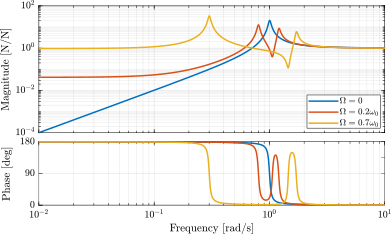
\includegraphics[scale=1]{figs/plant_iff_compare_rotating_speed.pdf}
\caption{\label{fig:plant_iff_compare_rotating_speed}Bode plot of \(\bm{G}_f\) for several rotational speeds \(\Omega\)}
\end{figure}


\subsection{Integral Force Feedback}
\label{sec:org049877c}

\begin{figure}[htbp]
\centering
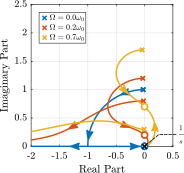
\includegraphics[scale=1]{figs/root_locus_pure_iff.pdf}
\caption{\label{fig:root_locus_pure_iff}Root Locus for the Decentralized Integral Force Feedback}
\end{figure}

At low frequency, the gain is very large and thus no force is transmitted between the payload and the rotating stage.
This means that at low frequency, the system is decoupled (the force sensor removed) and thus the system is unstable.


\section{Integral Force Feedback with High Pass Filters}
\label{sec:org54452db}
\subsection{Modification of the Control Low}
\label{sec:org325cdd4}


\subsection{Feedback Analysis}
\label{sec:org5efee77}

\begin{figure}[htbp]
\centering
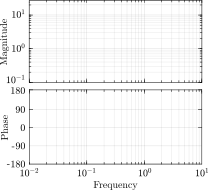
\includegraphics[scale=1]{figs/loop_gain_modified_iff.pdf}
\caption{\label{fig:loop_gain_modified_iff}Bode Plot of the Loop Gain for IFF with and without the HPF}
\end{figure}

\begin{figure}[htbp]
\centering
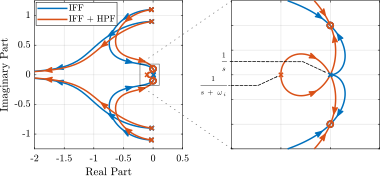
\includegraphics[scale=1]{figs/root_locus_modified_iff.pdf}
\caption{\label{fig:root_locus_modified_iff}Root Locus for IFF with and without the HPF}
\end{figure}

\subsection{Optimal Cut-Off Frequency}
\label{sec:orgd5828e4}

\begin{figure}[htbp]
\centering
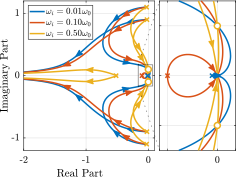
\includegraphics[scale=1]{figs/root_locus_wi_modified_iff.pdf}
\caption{\label{fig:root_locus_wi_modified_iff}Root Locus for several HPF cut-off frequencies \(\omega_i\)}
\end{figure}

\begin{figure}[htbp]
\centering
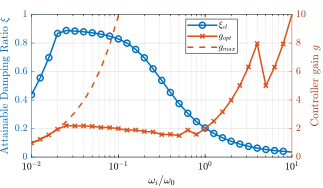
\includegraphics[scale=1]{figs/mod_iff_damping_wi.pdf}
\caption{\label{fig:mod_iff_damping_wi}Attainable damping ratio \(\xi_\text{cl}\) as a function of the HPF cut-off frequency. Corresponding control gain \(g_\text{opt}\) and \(g_\text{max}\) are also shown}
\end{figure}

\section{Integral Force Feedback with Parallel Springs}
\label{sec:org22884d6}
\subsection{Stiffness in Parallel with the Force Sensor}
\label{sec:orgb871bfd}

\begin{figure}[htbp]
\centering
\includegraphics[scale=1]{figs/system_parallel_springs.pdf}
\caption{\label{fig:system_parallel_springs}System with added springs \(k_p\) in parallel with the actuators}
\end{figure}


\subsection{Effect of the Parallel Stiffness on the Plant Dynamics}
\label{sec:org4d37cce}

\begin{figure}[htbp]
\centering
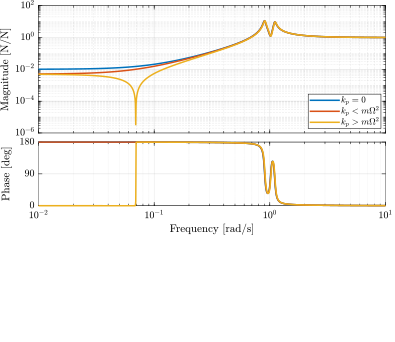
\includegraphics[scale=1]{figs/plant_iff_kp.pdf}
\caption{\label{fig:plant_iff_kp}Bode Plot of \(f_u/F_u\) without any parallel stiffness, with a parallel stiffness \(k_p < m \Omega^2\) and with \(k_p > m \Omega^2\)}
\end{figure}

\begin{figure}[htbp]
\centering
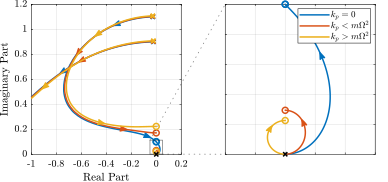
\includegraphics[scale=1]{figs/root_locus_iff_kp.pdf}
\caption{\label{fig:root_locus_iff_kp}Root Locus for IFF without any parallel stiffness, with a parallel stiffness \(k_p < m \Omega^2\) and with \(k_p > m \Omega^2\)}
\end{figure}


\subsection{Optimal Parallel Stiffness}
\label{sec:orgd19b212}

\begin{figure}[htbp]
\centering
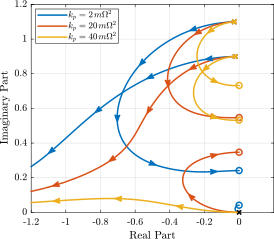
\includegraphics[scale=1]{figs/root_locus_iff_kps.pdf}
\caption{\label{fig:root_locus_iff_kps}Root Locus for IFF for several parallel spring stiffnesses \(k_p\)}
\end{figure}


\begin{figure}[htbp]
\centering
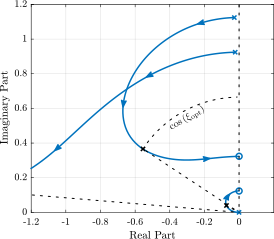
\includegraphics[scale=1]{figs/root_locus_opt_gain_iff_kp.pdf}
\caption{\label{fig:root_locus_opt_gain_iff_kp}Root Locus for IFF with \(k_p = 5 m \Omega^2\). The poles of the system using the gain that yields the maximum damping ratio are shown by black crosses}
\end{figure}

\section{Direct Velocity Feedback}
\label{sec:org6904969}
\subsection{Control Schematic}
\label{sec:org103e18b}

\begin{figure}[htbp]
\centering
\includegraphics[scale=1]{figs/system_dvf.pdf}
\caption{\label{fig:system_dvf}System with relative velocity sensors and with decentralized controllers \(K_V\)}
\end{figure}


\subsection{Equations}
\label{sec:org793c22d}



\subsection{Relative Direct Velocity Feedback}
\label{sec:orgc28d518}

\begin{figure}[htbp]
\centering
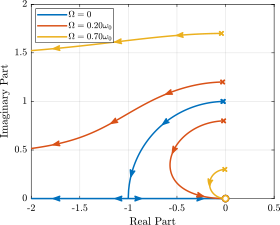
\includegraphics[scale=1]{figs/root_locus_dvf.pdf}
\caption{\label{fig:root_locus_dvf}Root Locus for Decentralized Direct Velocity Feedback for several rotational speeds \(\Omega\)}
\end{figure}

\section{Comparison of the Proposed Active Damping Techniques for Rotating Positioning Stages}
\label{sec:org6af1fdb}
\subsection{Physical Comparison}
\label{sec:orgdff3aa2}



\subsection{Attainable Damping}
\label{sec:org22c8f42}

\begin{figure}[htbp]
\centering
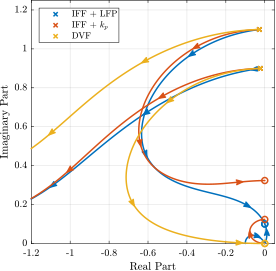
\includegraphics[scale=1]{figs/comp_root_locus.pdf}
\caption{\label{fig:comp_root_locus}Root Locus for the three proposed decentralized active damping techniques: IFF with HFP, IFF with parallel springs, and relative DVF}
\end{figure}


\subsection{Transmissibility and Compliance}
\label{sec:org3e2cf56}


\begin{figure}[htbp]
\begin{subfigure}[c]{0.45\linewidth}
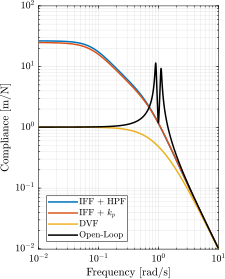
\includegraphics[width=\linewidth]{figs/comp_compliance.pdf}
\caption{\label{fig:comp_compliance} Transmissibility}
\end{subfigure}
\begin{subfigure}[c]{0.45\linewidth}
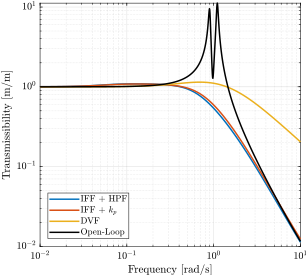
\includegraphics[width=\linewidth]{figs/comp_transmissibility.pdf}
\caption{\label{fig:comp_transmissibility} Compliance}
\end{subfigure}
\caption{\label{fig:comp_active_damping}Comparison of the three proposed Active Damping Techniques}
\centering
\end{figure}


\section{Conclusion}
\label{sec:orge292803}
\label{sec:conclusion}

\section*{Acknowledgment}
\label{sec:orgaf681fb}

\bibliography{ref.bib}
\end{document}
